\documentclass[../main.tex]{subfiles}
\begin{document}
	\chapter{Boundary conditions: specified nonzero value}
\label{chap:chap_14}
%\pagenumbering{arabic}
\setcounter{page}{90}
\noindent We have to take special actions to incorporate Dirichlet conditions, such as $u(L)=D$, into the computational procedures. The present section outlines alternative, yet mathematically equivalent, methods. \bigbreak
	\section[General construction of a boundary function]{General construction of a boundary function}
		\label{sec:sec_14_1}
		\noindent In Section \ref{sec:sec_11_11} we introduce a boundary function $B(x)$ to deal with nonzero Dirichlet boundary conditions for $u$. The construction of such a function is not always trivial, especially not in multiple dimensions. However, a simple and general construction idea exists when the basis functions have the property
		$$
		\varphi_{i}\left(x_{j}\right)=\delta_{i j}, \quad \delta_{i j}= \begin{cases}1, & i=j \\ 0, & i \neq j\end{cases}
		$$
		where $x_{j}$ is a boundary point. Examples on such functions are the Lagrange interpolating polynomials and finite element functions.
		
		Suppose now that $u$ has Dirichlet boundary conditions at nodes with numbers $i \in I_{b}$. For example, $I_{b}=\left\{0, N_{n}\right\}$ in a $1 \mathrm{D}$ mesh with node numbering from left to right. Let $U_{i}$ be the corresponding prescribed values of $u\left(x_{i}\right)$. We can then, in general, use
	
		\begin{equation}
			\label{eqa179}
			B(x)=\sum_{j \in I_{b}} U_{j} \varphi_{j}(x) .
		\end{equation}
	
		\noindent It is easy to verify that $B\left(x_{i}\right)=\sum_{j \in I_{b}} U_{j} \varphi_{j}\left(x_{i}\right)=U_{i}$.\smallbreak
		The unknown function can then be written as
		
		\begin{equation}
			\label{eqa180}
			u(x)=\sum_{j \in I_{b}} U_{j} \varphi_{j}(x)+\sum_{j \in \mathcal{I}_{s}} c_{j} 	\varphi_{\nu(j)}
		\end{equation}
	
		\noindent where $\nu(j)$ maps unknown number $j$ in the equation system to node $\nu(j)$. We can easily show that with this $u$, a Dirichlet condition $u\left(x_{k}\right)=U_{k}$ is fulfilled:
		$$
		u\left(x_{k}\right)=\sum_{j \in I_{b}} U_{j} \underbrace{\varphi_{j}(x)}_{\neq 0 \text { only for } j=k}+\sum_{j \in \mathcal{I}_{s}} c_{j} \underbrace{\varphi_{\nu(j)}\left(x_{k}\right)}_{=0, k \notin \mathcal{I}_{s}}=U_{k}
		$$
		
		Some examples will further clarify the notation. With a regular left-to-right numbering of nodes in a mesh with $\mathrm{P} 1$ elements, and Dirichlet conditions at $x=0$, we use finite element basis functions associated with the nodes $1,2, \ldots, N_{n}$, implying that $\nu(j)=j+1, j=0, \ldots, N$, where $N=N_{n}-1$. For the particular mesh below the expansion becomes
		$$
		u(x)=U_{0} \varphi_{0}(x)+c_{0} \varphi_{1}(x)+c_{1} \varphi_{2}(x)+\cdots+c_{4} \varphi_{5}(x) .
		$$
		
		\begin{figure}[H]
			\centering
			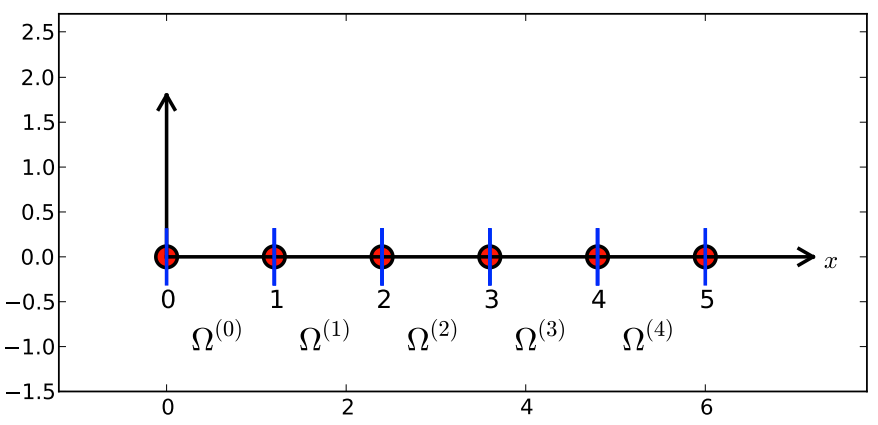
\includegraphics[width=0.7\linewidth]{img_48}
			\label{figi:img_48}
		\end{figure}
	
		Here is a mesh with an irregular cell and node numbering:
		
		\begin{figure}[H]
			\centering
			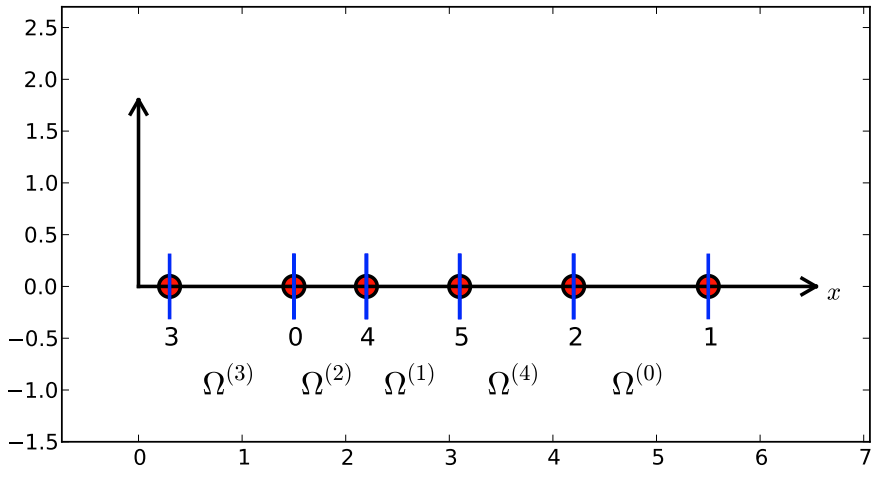
\includegraphics[width=0.7\linewidth]{img_49}
			\label{figi:img_49}
		\end{figure}
	
		Say we in this latter mesh have Dirichlet conditions on the left-most and right-most node, with numbers 3 and 1, respectively. Then we can number the unknowns at the interior nodes from left to right, giving $\nu(0)=0, \nu(1)=4$, $\nu(2)=5, \nu(3)=2$. This gives
		$$
		B(x)=U_{3} \varphi_{3}(x)+U_{1} \varphi_{1}(x),
		$$
		and
		$$
		u(x)=B(x)+\sum_{j=0}^{3} c_{j} \varphi_{\nu(j)}=U_{3} \varphi_{3}+U_{1} \varphi_{1}+c_{0} \varphi_{0}+c_{1} \varphi_{4}+c_{2} \varphi_{5}+c_{3} \varphi_{2}
		$$
		
		Switching to the more standard case of left-to-right numbering and boundary conditions $u(0)=C, u(L)=D$, we have $N=N_{n}-2$ and
		$$
		\begin{aligned}
			u(x) &=C \varphi_{0}+D_{\varphi_{n}}+\sum_{j \in I_{n}} c_{j} \varphi_{j+1} \\
			&=C \varphi_{0}+D_{\varphi_{N}}+c_{0} \varphi_{1}+c_{1} \varphi_{2}+\cdots+c_{N} \varphi_{N_{n}-1}
		\end{aligned}
		$$
		
		The idea of constructing $B$ described here generalizes almost trivially to $2 \mathrm{D}$ and 3D problems: $B=\sum_{j \in I_{b}} U_{j} \varphi_{j}$, where $I_{b}$ is the index set containing the numbers of all the nodes on the boundaries where Dirichlet values are prescribed.
		
	\section[Example on computing with finite element-based a boundary function]{Example on computing with finite element-based a boundary function}
		\label{sec:sec_14_2}
		\noindent Let us see how the model problem $-u^{\prime \prime}=2, u(0)=C, u(L)=D$, is affected by a $B(x)$ to incorporate boundary values. Inserting the expression
		$$
		u(x)=B(x)+\sum_{j \in \mathcal{I}_{x}} c_{j} \psi_{j}(x)
		$$
		in $-\left(u^{\prime \prime}, \psi_{i}\right)=\left(f, \psi_{i}\right)$ and integrating by parts results in a linear system with
		$$
		A_{i, j}=\int_{0}^{L} \psi_{i}^{\prime}(x) \psi_{j}^{\prime}(x) \mathrm{d} x, \quad b_{i}=\int_{0}^{L}\left(f(x)-B^{\prime}(x)\right) \psi_{i}(x) \mathrm{d} x
		$$
		We choose $\psi_{i}=\varphi_{i+1}, i=0, \ldots, N=N_{n}-2$ if the node numbering is from left to right. (Later we also need the assumption that the cells too are numbered from left to right.) The boundary function becomes
		$$
		B(x)=C \varphi_{0}(x)+D \varphi_{N_{n}}(x) .
		$$
		The expansion for $u(x)$ is
		$$
		u(x)=B(x)+\sum_{j \in \mathcal{I}_{x}} c_{j} \varphi_{j+1}(x) .
		$$
		We can write the matrix and right-hand side entries as
		$$
		A_{i-1, j-1}=\int_{0}^{L} \varphi_{i}^{\prime}(x) \varphi_{j}^{\prime}(x) \mathrm{d} x, \quad b_{i-1}=\int_{0}^{L}\left(f(x)-C \varphi_{0}^{\prime}(x)-D \varphi_{N_{\mathrm{m}}}^{\prime}(x)\right) \varphi_{i}(x) \mathrm{d} x
		$$
		for $i, j=1, \ldots, N+1=N_{n}-1$. Note that we have here used $B^{\prime}=C \varphi_{0}^{\prime}+D_{\varphi^{\prime}} N_{n}$.\bigbreak
		\textbf{Computations in physical coordinates.   } Most of the terms in the linear system have already been computed so we concentrate on the new contribution from the boundary function. The integral $\left.C \int_{0}^{L} \varphi_{0}^{\prime}(x)\right) \varphi_{i}(x) \mathrm{d} x$ can only get a nonzero contribution from the first cell, $\Omega^{(0)}=\left[x_{0}, x_{1}\right]$ since $\varphi_{0}^{\prime}(x)=0$ on all other cells. Moreover, $\varphi_{0}^{\prime}(x) \varphi_{i}(x) \mathrm{d} x \neq 0$ only for $i=0$ and $i=1$ (but $i=0$ is excluded), since $\varphi_{i}=0$ on the first cell if $i>1$. With a similar reasoning we realize that $\left.D \int_{0}^{L} \varphi_{N_{n}}^{\prime}(x)\right) \varphi_{i}(x) \mathrm{d} x$ can only get a nonzero contribution from the last cell. From the explanations of the calculations in Section \ref{sec:sec_3_6} we then find that
		$$
		\int_{0}^{L} \varphi_{0}^{\prime}(x) \varphi_{1}(x) \mathrm{d} x=\frac{1}{h} \cdot \frac{1}{h}=-\frac{1}{2}, \quad \int_{0}^{L} \varphi_{N_{n}}^{\prime}(x) \varphi_{N_{n}-1}(x) \mathrm{d} x=\frac{1}{h} \cdot \frac{1}{h}=\frac{1}{2}
		$$
		The extra boundary term because of $B(x)$ boils down to adding $C / 2$ to $b_{0}$ and $-D / 2$ to $b_{N}$.\bigbreak 
		
		\noindent \textbf{Cellwise computations on the reference element.   } As an equivalent alternative, we now turn to cellwise computations. The element matrices and vectors are calculated as Section \ref{sec:sec_13_4}, so we concentrate on the impact of the new term involving $B(x)$. We observe that $C \varphi_{0}^{\prime}=0$ on all cells except $e=0$, and $D \varphi_{N_{n}}^{\prime}=0$ on all cells except $e=N_{e}$. In this case there is only one unknown in these cells since $u(0)$ and $u(L)$ are prescribed, so the element vector has only one entry. The entry for the last cell, $e=N_{c}$, becomes
		$$
		\bar{b}_{0}^{(e)}=\int_{-1}^{1}\left(f-D \frac{2}{h} \frac{d \bar{\varphi}_{1}}{d X}\right) \bar{\varphi}_{0} \frac{h}{2} \mathrm{~d} X=\left(\frac{h}{2}\left(2-D \frac{2}{h} \frac{1}{2}\right) \int_{-1}^{1} \bar{\varphi}_{0} \mathrm{~d} X=h-D / 2\right.
		$$
		Similar computations on the first cell yield
		$$
		\tilde{b}_{0}^{(0)}=\int_{-1}^{1}\left(f-C \frac{2}{h} \frac{d \bar{\varphi}_{0}}{d X}\right) \bar{\varphi}_{1} \frac{h}{2} \mathrm{~d} X=\left(\frac{h}{2}\left(2+C \frac{2}{h} \frac{1}{2}\right) \int_{-1}^{1} \bar{\varphi}_{1} \mathrm{~d} X=h+C / 2\right.
		$$
		When assembling these contributions, we see that $b_{0}$ gets right-hand side of the linear system gets an extra term $C / 2$ and $b_{N}$ gets $-D / 2$, as in the computations in the physical domain.\bigbreak 
	
	\section[Modification of the linear system]{Modification of the linear system}
		\label{sec:sec_14_3}
		\noindent From an implementational point of view, there is a convenient alternative to adding the $B(x)$ function and using only the basis functions associated with nodes where $u$ is truly unknown. Instead of seeking
		
		\begin{equation}
			\label{eqa181}
			u(x)=\sum_{j \in I_{b}} U_{j} \varphi_{j}(x)+\sum_{j \in I_{a}} c_{j} \varphi_{\nu(j)}(x)
		\end{equation}
	
		\noindent we use the sum over all degrees of freedom, including the known boundary values:
		
		\begin{equation}
			\label{eqa182}
			u(x)=\sum_{j \in \mathcal{I}_{s}} c_{j} \varphi_{j}(x) .
		\end{equation}
	
		\noindent Note that the collections of unknowns $\left\{c_{i}\right\}_{i \in \mathcal{I}_{s}}$ in (\ref{eqa181}) and (\ref{eqa182}) are different: in (\ref{eqa181}) $N$ counts the number of nodes where $u$ is not known, while in (\ref{eqa181}) $N$ counts all the nodes $\left(N=N_{n}\right)$.
		
		The idea is to compute the entries in the linear system as if no Dirichlet values are prescribed. Afterwards, we modify the linear system to ensure that the known $c_{j}$ values are incorporated.
		
		A potential problem arises for the boundary term $\left[u^{\prime} v\right]_{0}^{L}$ from the integration by parts: imagining no Dirichlet conditions means that we no longer require $v=0$ at Dirichlet points, and the boundary term is then nonzero at these points. However, when we modify the linear system, we will erase whatever the contribution from $\left[u^{\prime} v\right]_{0}^{L}$ should be at the Dirichlet points in the right-hand side of the linear system. We can therefore safely forget $\left[u^{\prime} v\right]_{0}^{L}$ at any point where a Dirichlet condition applies.\bigbreak
		
		\noindent \textbf{Computations in the physical system.   } Let us redo the computations in the example in Section \ref{sec:sec_14_1}. We solve $-u^{\prime \prime}=2$ with $u(0)=0$ and $u(L)=D$. The expressions for $A_{i, j}$ and $b_{i}$ are the same, but the numbering is different as the numbering of unknowns and nodes now coincide:
		$$
		A_{i, j}=\int_{0}^{L} \varphi_{i}^{\prime}(x) \varphi_{j}^{\prime}(x) \mathrm{d} x, \quad b_{i}=\int_{0}^{L} f(x) \varphi_{i}(x) \mathrm{d} x
		$$
		for $i, j=0, \ldots, N=N_{n}$. The integrals involving basis functions corresponding to interior mesh nodes, $i, j=1, \ldots, N_{n}-1$, are obviously the same as before. We concentrate on the contributions from $\varphi_{0}$ and $\varphi_{N_{n}}$ :
		$$
		\begin{aligned}
			A_{0,0} &=\int_{0}^{L}\left(\varphi_{0}^{\prime}\right)^{2} \mathrm{~d} x=\int_{0}^{x_{1}}=\left(\varphi_{0}^{\prime}\right)^{2} \mathrm{~d} x \frac{1}{h} \\
			A_{0,1} &=\int_{0}^{L} \varphi_{0}^{\prime} \varphi_{1}^{\prime} \mathrm{d} x=\int_{0}^{x_{1}} \varphi_{0}^{\prime} \varphi_{1}^{\prime} \mathrm{d} x=-\frac{1}{h} \\
			A_{N, N} &=\int_{0}^{L}\left(\varphi_{0}^{\prime}\right)^{2} \mathrm{~d} x=\int_{x_{N_{n}-1}}^{x_{n}}\left(\varphi_{0}^{\prime}\right)^{2} \mathrm{~d} x=\frac{1}{h} \\
			A_{N, N-1} &=\int_{0}^{L}\left(\varphi_{0}^{\prime}\right)^{2} \mathrm{~d} x=\int_{x_{N_{n}-1}}\left(\varphi_{0}^{\prime}\right)^{2} \mathrm{~d} x=-\frac{1}{h}
		\end{aligned}
		$$
		The new terms on the right-hand side are also those involving $\varphi_{0}$ and $\varphi_{N_{n}}$ :
		$$
		\begin{aligned}
			b_{0} &=\int_{0}^{L} 2 \varphi_{0}(x) \mathrm{d} x=\int_{0}^{x_{1}} 2 \varphi_{0}(x) \mathrm{d} x=h, \\
			b_{N} &=\int_{0}^{L} 2 \varphi_{N_{n}} \mathrm{~d} x=\int_{x_{N_{n}-1}}^{x_{N_{n}}} 2 \varphi_{N_{n}} \mathrm{~d} x=h .
		\end{aligned}
		$$
		The complete matrix system, involving all degrees of freedom, takes the form
		\begin{equation}
			\label{eqa183}
			\frac{1}{h}\left(\begin{array}{ccccccccc}
				1 & -1 & 0 & \cdots & \cdots & \cdots & \cdots & \cdots & 0 \\
				-1 & 2 & -1 & \ddots & & & & & \vdots \\
				0 & -1 & 2 & -1 & \ddots & & & & \vdots \\
				\vdots & \ddots & & \ddots & \ddots & 0 & & & \vdots \\
				\vdots & & \ddots & \ddots & \ddots & \ddots & \ddots & & \vdots \\
				\vdots & & & 0 & -1 & 2 & -1 & \ddots & \vdots \\
				\vdots & & & & \ddots & \ddots & \ddots & \ddots & 0 \\
				\vdots & & & & & \ddots & \ddots & \ddots & -1 \\
				0 & \ldots & \ldots & \cdots & \cdots & \cdots & 0 & -1 & 1
			\end{array}\right)\left(\begin{array}{c}
				c_{0} \\
				\vdots \\
				\vdots \\
				\vdots \\
				\vdots \\
				\vdots \\
				\vdots \\
				\vdots \\
				c_{N}
			\end{array}\right)=\left(\begin{array}{c}
				h \\
				2 h \\
				\vdots \\
				\vdots \\
				\vdots \\
				\vdots \\
				\vdots \\
				2 h \\
				h
			\end{array}\right)
		\end{equation}
	
		Incorporation of Dirichlet values can now be done by replacing the first and last equation by $c_{0}=0$ and $c_{N}=D$. This action changes the system to
		
	\begin{equation}
		\label{eqa184}	
		\frac{1}{h}\left(\begin{array}{ccccccccc}
			h & 0 & 0 & \cdots & \cdots & \cdots & \cdots & \cdots & 0 \\
			-1 & 2 & -1 & \ddots & & & & & \vdots \\
			0 & -1 & 2 & -1 & \ddots & & & & \vdots \\
			\vdots & \ddots & & \ddots & \ddots & 0 & & & \vdots \\
			\vdots & & \ddots & \ddots & \ddots & \ddots & \ddots & & \vdots \\
			\vdots & & & 0 & -1 & 2 & -1 & \ddots & \vdots \\
			\vdots & & & & \ddots & \ddots & \ddots & \ddots & 0 \\
			\vdots & & & & & \ddots & \ddots & \ddots & -1 \\
			0 & \cdots & \cdots & \cdots & \cdots & \cdots & 0 & 0 & h
		\end{array}\right)\left(\begin{array}{c}
			c_{0} \\
			\vdots \\
			\vdots \\
			\vdots \\
			\vdots \\
			\vdots \\
			\vdots \\
			\vdots \\
			c_{N}
		\end{array}\right)=\left(\begin{array}{c}
			0 \\
			2 h \\
			\vdots \\
			\vdots \\
			\vdots \\
			\vdots \\
			\vdots \\
			2 h \\
			D
		\end{array}\right)
	\end{equation}

		Note that because we do not require $\varphi_{i}(0)=0$ and $\varphi_{i}(L), i \in \mathcal{I}_{s}$, the boundary term $\left[u^{\prime} v\right]_{0}^{L}$ gives in principle contributions $u^{\prime}(0) \varphi_{0}(0)$ to $b_{0}$ and $u^{\prime}(L) \varphi_{N}(L)$ to $b_{N}\left(u^{\prime} \varphi_{i}\right.$ vanishes for $x=0$ or $x=L$ for $\left.i=1, \ldots, N-1\right)$. Nevertheless, we erase these contributions in $b_{0}$ and $b_{N}$ and insert boundary values instead. This argument shows why we can drop computing $\left[u^{\prime} v\right]_{0}^{L}$ at Dirichlet nodes when we implement the Dirichlet values by modifying the linear system.
		
	\section[Symmetric modification of the linear system]{Symmetric modification of the linear system}
		\label{sec:sec_14_4}
		The original matrix system (\ref{eqa172}) is symmetric, but the modifications in (\ref{eqa184}) destroy the symmetry. Our described modification will in general destroy an initial symmetry in the matrix system. This is not a particular computational disadvantage for tridiagonal systems arising in $1 \mathrm{D}$ problems, but may be more serious in $2 \mathrm{D}$ and 3D problems when the systems are large and exploiting symmetry can be important for halving the storage demands, speeding up computations, and/or making the solution algorithm more robust. Therefore, an alternative modification which preserves symmetry is frequently applied.\smallbreak
		Let $c_{k}$ be a coefficient corresponding to a known value $u\left(x_{k}\right)=U_{k}$. We want to replace equation $k$ in the system by $c_{k}=U_{k}$, i.e., insert zeroes in row number $k$ in the coefficient matrix, set 1 on the diagonal, and replace $b_{k}$ by $U_{k}$. A symmetry-preserving modification consists in first subtracting column number $k$ in the coefficient matrix, i.e., $A_{i, k}$ for $i \in \mathcal{I}_{s}$, times the boundary value $U_{k}$, from the right-hand side: $b_{i} \leftarrow b_{i}-A_{i, k} U_{k}$. Then we put zeroes in row number $k$ and column number $k$ in the coefficient matrix, and finally set $b_{k}=U_{k}$. The steps in algorithmic form becomes
		\begin{enumerate}
			\item $b_{i} \leftarrow b_{i}-A_{i, k} U_{k}$ for $i \in \mathcal{I}_{s}$ \bigbreak
			\item $A_{i, k}=A_{k, i}=0$ for $i \in \mathcal{I}_{s}$ \bigbreak
			\item $A_{k, k}=1$ \bigbreak
			\item $b_{i}=U_{k}$ \bigbreak
		\end{enumerate}
		
		\noindent This modification goes as follows for the specific linear system written out in (\ref{eqa183}) in Section \ref{sec:sec_14_3}. First we subtract the first column in the coefficient matrix, times the boundary value, from the right-hand side. Because $c_{0}=0$, this subtraction has no effect. Then we subtract the last column, times the boundary value $D$, from the right-hand side. This action results in $b_{N-1}=2 h+D / h$ and $b_{N}=h-2 D / h$. Thereafter, we place zeros in the first and last row and column in the coefficient matrix and 1 on the two corresponding diagonal entries. Finally, we set $b_{0}=0$ and $b_{N}=D$. The result becomes
		
		\begin{equation}
			\label{eqa185}	
			\frac{1}{h}\left(\begin{array}{ccccccccc}
				h & 0 & 0 & \cdots & \cdots & \cdots & \cdots & \cdots & 0 \\
				0 & 2 & -1 & \ddots & & & & & \vdots \\
				0 & -1 & 2 & -1 & \ddots & & & & \vdots \\
				\vdots & \ddots & & \ddots & \ddots & 0 & & & \vdots \\
				\vdots & & \ddots & \ddots & \ddots & \ddots & \ddots & & \vdots \\
				\vdots & & & 0 & -1 & 2 & -1 & \ddots & \vdots \\
				\vdots & & & & \ddots & \ddots & \ddots & \ddots & 0 \\
				\vdots & & & & & \ddots & \ddots & \ddots & 0 \\
				0 & \cdots & \cdots & \cdots & \cdots & \cdots & 0 & 0 & h
			\end{array}\right)\left(\begin{array}{c}
				c_{0} \\
				\vdots \\
				\vdots \\
				\vdots \\
				\vdots \\
				\vdots \\
				\vdots \\
				\vdots \\
				c_{N}
			\end{array}\right)=\left(\begin{array}{c}
				0 \\
				2 h \\
				\vdots \\
				\vdots \\
				\vdots \\
				\vdots \\
				\vdots \\
				2 h + D/h \\
				D
			\end{array}\right)
		\end{equation}
	\bigbreak
	\section[Modification of the element matrix and vector]{Modification of the element matrix and vector}
		\noindent The modifications of the global linear system can alternatively be done for the element matrix and vector. (The assembled system will get the value $n$ on the main diagonal if $n$ elements contribute to the same unknown, but the factor $n$ will also appear on the right-hand side and hence cancel out.)
		
		We have, in the present computational example, the element matrix and vector (\ref{eqa177}). The modifications are needed in cells where one of the degrees of freedom is known. Here, this means the first and last cell. We compute the element matrix and vector as there are no Dirichlet conditions. The boundary term $\left[u^{\prime} v\right]_{0}^{L}$ is simply forgotten at nodes that have Dirichlet conditions because the modification of the element vector will anyway erase the contribution from the boundary term. In the first cell, local degree of freedom number 0 is known and the modification becomes
		\begin{equation}
			\label{eqa186}	
			\tilde{A}^{(0)}=A=\frac{1}{h}\left(\begin{array}{rr}
				h & 0 \\
				-1 & 1
			\end{array}\right), \quad \tilde{b}(0)=\left(\begin{array}{l}
				0 \\
				h
			\end{array}\right)
		\end{equation}
		In the last cell we set
		\begin{equation}
			\label{eqa187}
			\bar{A}^{\left(N_{e}\right)}=A=\frac{1}{h}\left(\begin{array}{rr}
				1 & -1 \\
				0 & h
			\end{array}\right), \quad \vec{b}^{\left(N_{c}\right)}=\left(\begin{array}{l}
				h \\
				D
			\end{array}\right)
		\end{equation}
	
		We can also perform the symmetric modification. This operation affects only the last cell with a nonzero Dirichlet condition. The algorithm is the same as for the global linear system, resulting in
		\begin{equation}
			\label{eqa188}
			\tilde{A}^{(N-1)}=A=\frac{1}{h}\left(\begin{array}{cc}
				h & 0 \\
				0 & 1
			\end{array}\right), \quad \tilde{b}^{(N-1)}=\left(\begin{array}{c}
				h+D / h \\
				D
			\end{array}\right) .
		\end{equation}
		The reader is encouraged to assemble the element matrices and vectors and check that the result coincides with the system (\ref{eqa185}).
\clearpage
\end{document} 
